\documentclass{beamer}
\usepackage[english]{babel}
\usepackage{amsmath,amsthm}
\usepackage{amsfonts}
\usepackage{graphicx}

% SET THEME AND COLOUR SCHEME
\usetheme[secheader]{Boadilla}
\usecolortheme{crane}

% GROUP-SPECIFIC INFORMATION
\title[Short title]{Full title}
\author[]{Author 1 \and Author 2 \and Author 3 \and Author 4}
\date{June 18, 2015}
\institute[Stokes Workshop]{2nd Annual Stokes Modelling Workshop}



\begin{document}

\frame{\titlepage}


\section{Problem description}



\frame {
    \frametitle{Bullet points and lists}


\begin{itemize}
\item Point 1
\item Point 2
\item Point 3
\end{itemize}

\begin{enumerate}
\item Point 1
\item Point 2
\item Point 3
\end{enumerate}


}


\frame {
    \frametitle{Staggered bullet points}


\begin{itemize}
\item<1-> Point 1
\item<2-> Point 2
\item<3-> Point 3
\end{itemize}


}



\section{Results}



\frame {
    \frametitle{Sample equations}

\begin{equation*}
\frac{\partial M}{\partial t} + \frac{\partial M}{\partial x}  =  g(M).
\end{equation*}

\begin{eqnarray*}
\frac{d x}{dt}  & = & a x, \\
\frac{d y}{dt}  & = & b x + c y^2,
\end{eqnarray*}

}



\frame {
    \frametitle{Sample image and text}

\begin{center}

\begin{figure}
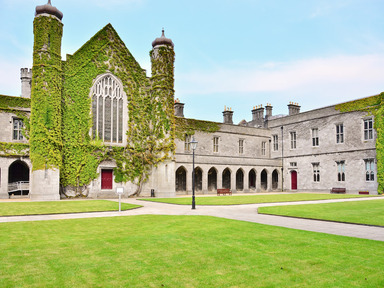
\includegraphics[width=0.5\textwidth]{quad.png}
\end{figure}

{\small Small text} \\

{\Large Large text} \\

\end{center}

}



\frame {
    \frametitle{Sample bibliography}

\begin{thebibliography}{SW15}

\bibitem[]{ref1}
P. Rohani, O. Miramontes, M.~P. Hassell
\newblock Quasiperiodicity and chaos in
  population models.
\newblock {\em Proceedings of the Royal Society of London B}, 258(1351):17--22, 1994.

\end{thebibliography}


}


\end{document}